\section{Introduction}

Vision-and-language navigation (VLN) asks an agent to follow a written route instruction through a
building, seeing only what its own camera sees. In Room-to-Room in Continuous Environments (R2R-CE)
\citep{anderson2018r2r,krantz2020beyond}, the agent has four actions at every step: move forward
0.25 m, turn left or right by 15 degrees, or stop. An episode counts as a success only if the agent
itself stops within 3 m of the goal. Stopping is a spatial judgment: the agent must recognize from
its own view that it has reached a place described only in words. We report Success Rate (SR), the
share of episodes that end this way, and Oracle Success (OSR), the share whose path ever enters the
goal radius, whether or not the agent stops there.

Fine-tuning a navigation policy saves a series of checkpoints, and one of them must be chosen. The
direct way to choose is a closed-loop rollout: run each checkpoint in the simulator, where every
action it takes determines what it sees next, and count its successes. Rollouts are expensive, but
without them a general-purpose fine-tuning pipeline can still compute one number per checkpoint, its
validation loss. Asked to keep its best checkpoint, the Hugging Face Trainer keeps the one with the
lowest evaluation loss unless given another metric \citep{hf2026trainer}. For a navigation policy
this loss is teacher-forced. At each held-out step the model sees the expert's own past frames, and
it is scored by the cross-entropy (CE) of the expert's next action.

In R2R-CE, this loss averages over decisions in which one action dominates. Of the 631{,}244
decisions in the released training split, $64.1\%$ are \textsc{move\_forward}. Among the 197{,}455
decisions eligible for this study, $66.6\%$ are \textsc{move\_forward} and only $1.76\%$ are
\textsc{stop}. The average can therefore improve while the model stops predicting \textsc{stop}, the
action that success requires. Figure~\ref{fig:selection_schematic} shows a case from our experiments.
The checkpoint the loss selects is scored on $256$ held-out decisions, only three of which call for
\textsc{stop}. In $61$ episodes in the simulator, it never stops. We call this failure mode
\textsc{StopBlind}: when \textsc{stop} is only a few percent of the decisions that a selection loss
averages, the loss can rank best a checkpoint that never stops at the goal, and it gives no sign of
whether any checkpoint does.

\citet{xiang2020l2stop} pointed out that an unweighted loss gives \textsc{stop} too little
attention. \citet{wijmans2019eqa} warned that navigation policies can reach very high validation
accuracy on action prediction while missing every change of action. Executing five low-loss
checkpoints per model in embodied question answering, they found that a loss weighted toward those
changes predicted end-to-end performance better than plain cross-entropy. Failures to stop have been
documented for VLN agents on a discrete navigation graph \citep{zhao2023mindthegap} and reported for
a vision--language model (VLM) fine-tuned for R2R-CE \citep{dang2026rynnbrain}. To our knowledge, no
one has measured which checkpoint the loss selects for a VLM policy in continuous R2R-CE, or whether
it passes over a better one.

We fine-tune Qwen3-VL-8B, an open VLM, with and without class weighting, three seeds each. Class
weighting multiplies each decision's loss by the inverse of its action's training frequency, so that
rare actions count more. We run every selected checkpoint in the simulator on a frozen set of 61
episodes from \texttt{val\_seen}, the validation split whose buildings also appear in training, under
the official 500-step cap. We compare each run with an always-forward baseline, a policy that moves
forward at every step. Before the first run, we also fixed a pass/fail test, the existence gate,
which asks whether a model learned more than how often each action occurs and whether it recalls
\textsc{stop} (Section~\ref{sec:data}). In a preregistered follow-up, we then execute all 37
distinct saved checkpoints to test whether the rule passed over a better one. Its analysis and the
bar a checkpoint must clear were fixed before any unselected checkpoint was run or scored. The study covers
one model, one training budget of 192 updates, and buildings seen in training. Three single-seed
probes, which supervise four-action chunks, scale the data 44$\times$, or add metric 3D geometry,
change the policies' behavior but cannot test stopping, because their data loader dropped every
decision whose target was \textsc{stop}. Our contributions are:
\begin{enumerate}[leftmargin=1.4em,topsep=2pt,itemsep=1pt]
  \item \textbf{Without class weighting, the validation loss selects policies that never stop.} In
  all three unweighted runs, the loss selects the same checkpoint, update 160 of 192. It predicts
  \textsc{stop} on none of the $256$ held-out decisions used to select it, and on none of the $64$
  \textsc{stop} decisions in a separate held-out set. In the simulator, two of these checkpoints take the same actions as the
  always-forward baseline, and the third differs in one episode.
  \item \textbf{Class weighting changes which action is repeated, and the policies still fail.}
  Weighted policies use all four actions in aggregate, but most episodes repeat one action
  throughout, and every \textsc{stop} they press is outside the goal radius.
  \item \textbf{No selected checkpoint succeeds, and no other was shown to do better.} All six
  selected checkpoints have SR $0/61$. Of all 37 distinct saved checkpoints, one succeeds in one
  episode: the untrained model, $1/61$. No candidate reaches the preregistered bar against its run's
  selected checkpoint.
  \item \textbf{Per-class checks detect the failure offline.} Recall on \textsc{stop} and the
  existence gate flag all six selected runs before any simulator run, and none of the 37 checkpoints
  passes the gate.
\end{enumerate}

\begin{figure}[t]
  \centering
  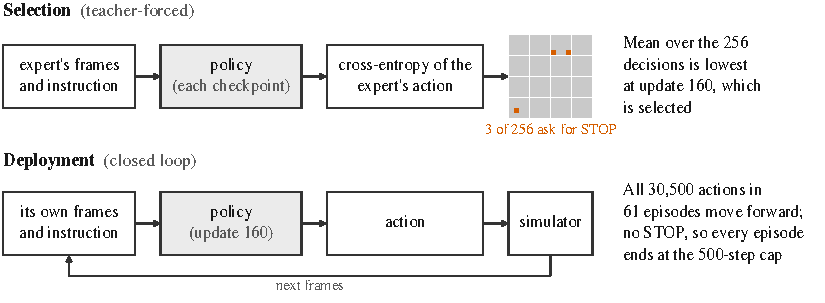
\includegraphics[width=\linewidth]{figures/p1_selection_schematic.pdf}
  \caption{\textbf{Checkpoint selection compared with deployment.} Selection scores each
  of $256$ held-out decisions with the expert's history supplied, and picks update $160$. Deployment
  runs that checkpoint on $61$ episodes under the $500$-step cap, where its own action sets the next
  observation. All $30{,}500$ actions it takes are \textsc{move\_forward}, although three of the
  $256$ scored decisions ask for \textsc{stop}. Shown for unweighted seed $20260826$. The weighted
  runs behave differently (Table~\ref{tab:closed-loop-behavior}).}
  \label{fig:selection_schematic}
\end{figure}
